\section*{Introduction}

We propose a reference implementation of \citep{Guthrie:2013} that introduces an
action selection mechanism in cortico-basal ganglia loops based on a
competition between the positive feedback, direct pathway through the striatum
and the negative feedback, hyperdirect pathway through the subthalamic
nucleus. The original implementation was made in Delphi (Object Pascal) whose
sources are available on request to any of the author of the original
article. We have used these sources to disambiguate ambiguous and missing
information in the original article. The reference implementation we propose
has been coded in Python for ease of reading and Cython for performances
because the main result includes a batch of 250 experiments over 120 trials
that would be too slow for regular Python scripts.


\section*{Methods}

We used the description of the model in the original article as well as the
sources of the model (requested from author) that are made of hundred files and
6,000 lines of Delphi for the main source. We've been unable to compile this
original implementation but we're able to run the provided Windows executable.
We found some factual errors in the original article that have been corrected
in this implementation. We provide below the formal description of the model
according to the proposition of \cite{Nordlie:2009} for reproducible
descriptions of neuronal network models.

\begin{table}[htbp]
  \small \sffamily \centering
  \begin{tabular}{ll}
\bf Table & \bf Description\\
\hline 
Populations & Cortex (motor, associative \& cognitive),\\
            & Striatum (motor, associative \& cognitive),\\
            & GPi (motor \& cognitive),\\
            & STN (motor \& cognitive),\\
            & Thalamus (motor \& cognitive)\\
Topology & --\\
Connectivity & One to one, one to many (divergent), many to one (convergent)\\
Neuron model & Dynamic rate model\\
Channel model & --\\
Synapse model & Linear synapse\\
Plasticity & Reinforcement learning rule\\
Input & External current in cortical areas (motor, associative \& cognitive)\\
Recordings & Firing rate \& performances\\
\hline
  \end{tabular}
\caption{Model description following \cite{Nordlie:2009} prescription.}
\end{table}


\begin{table}[htbp]
  \small \sffamily \centering
  \begin{tabular}{llllll}
\bf Name & \bf Elements & \bf Size & \bf Threshold & \bf Noise & \bf Initial state\\
\hline
Cortex motor & Linear neuron & \(1 \times 4\) & -3 & 1.0\% & 0.0\\
Cortex cognitive & Linear neuron & \(4 \times 1\) & -3 & 1.0\% & 0.0\\
Cortex associative & Linear neuron & \(4 \times 4\) & -3 & 1.0\% & 0.0\\
Striatum motor & Sigmoidal neuron & \(1 \times 4\) & 0 & 0.1\% & 0.0\\
Striatum cognitive & Sigmoidal neuron & \(4 \times 1\) & 0 & 0.1\% & 0.0\\
Striatum associative & Sigmoidal neuron & \(4 \times 4\) & 0 & 0.1\% & 0.0\\
GPi motor & Linear neuron & \(1 \times 4\) & +10 & 3.0\% & 0.0\\
GPi cognitive & Linear neuron & \(4 \times 1\) & +10 & 3.0\% & 0.0\\
STN motor & Linear neuron & \(1 \times 4\) & -10 & 0.1\% & 0.0\\
STN cognitive & Linear neuron & \(4 \times 1\) & -10 & 0.1\% & 0.0\\
Thalamus motor & Linear neuron & \(1 \times 4\) & -40 & 0.1\% & 0.0\\
Thalamus cognitive & Linear neuron & \(4 \times 1\) & -40 & 0.1\% & 0.0\\
Values (\(V_i\)) & Scalar & \(4\) & -- & -- & 0.5\\
\hline
\end{tabular}
\caption{Populations}
\end{table}

\begin{table}[htbp]
  \small \sffamily \centering
  \begin{tabular}{llllll}
\bf Source & \bf Target & \bf Pattern & \bf Weight & \bf Gain & \bf Plastic\\
\hline
Cortex motor & Thalamus motor & \((1,i) \rightarrow (1,i)\) & 1.0 & 0.4 & No\\
Cortex cognitive & Thalamus cognitive & \((i,1) \rightarrow (i,1)\) & 1.0 & 0.4 & No\\
Cortex motor & STN motor & \((1,i) \rightarrow (1,i)\) & 1.0 & 1.0 & No\\
Cortex cognitive & STN cognitive & \((i,1) \rightarrow (i,1)\) & 1.0 & 1.0 & No\\
Cortex motor & Striatum motor & \((1,i) \rightarrow (1,i)\) & 0.5 & 1.0 & No\\
Cortex cognitive & Striatum cognitive & \((i,1) \rightarrow (i,1)\) & 0.5 & 1.0 & Yes\\
Cortex motor & Striatum associative & \((1,i) \rightarrow (.,i)\) & 0.5 & 0.2 & No\\
Cortex cognitive & Striatum associative & \((i,1) \rightarrow (i,.)\) & 0.5 & 0.2 & No\\
Cortex associative & Striatum associative & \((i,j) \rightarrow (i,j)\) & 0.5 & 1.0 & No\\
Thalamus motor & Cortex motor & \((1,i) \rightarrow (1,i)\) & 1.0 & 1.0 & No\\
Thalamus cognitive & Cortex cognitive & \((i,1) \rightarrow (i,1)\) & 1.0 & 1.0 & No\\
GPi motor & Thalamus motor & \((1,i) \rightarrow (1,i)\) & 1.0 & -0.5 & No\\
GPi cognitive & Thalamus cognitive & \((i,1) \rightarrow (i,1)\) & 1.0 & -0.5 & No\\
STN motor & GPi motor & \((1,i) \rightarrow (1,i)\) & 1.0 & 1.0 & No\\
STN cognitive & GPi cognitive & \((i,1) \rightarrow (i,1)\) & 1.0 & 1.0 & No\\
Striatum cognitive & GPi cognitive & \((i,1) \rightarrow (i,1)\) & 1.0 & -2.0 & No\\
Striatum motor & GPi motor & \((i,1) \rightarrow (i,1)\) & 1.0 & -2.0 & No\\
Striatum associative & GPi motor & \((.,i) \rightarrow (1,i)\) & 1.0 & -2.0 & No\\
Striatum associative & GPi cognitive & \((i,.) \rightarrow (i,1)\) & 1.0 & -2.0 & No\\
\hline
\end{tabular}
\caption{Connectivity}
\end{table}




\begin{table}[htbp]
\small \sffamily \centering
\begin{tabular}{ll}
\bf Linear neuron &\\
\hline
Type               & Rate model\\
Membrane Potential & \(\tau dV/dt = -V + I_{syn} + I_{ext} - h\)\\
                   & \(U = max(V,0)\)\\
\hline
\end{tabular}
\caption{Neuron Model (1)}
\end{table}



\begin{table}[htbp]
\small \sffamily \centering
\begin{tabular}{ll}
\bf Sigmoidal neuron &\\
\hline
Type & Rate model\\
Membrane Potential & \(\tau dV/dt = -V + I_{syn} + I_{ext} - h\)\\
&\(U = V_{min} - (V_{max}-V_{min}) / \left(1+e^{\frac{V_h - V}{V_c}}\right)\)\\
\hline
\end{tabular}
\caption{Neuron Model (2)}
\end{table}



\begin{table}[htbp]
\small\sffamily \centering
\begin{tabular}{ll}
\bf Linear synapse &\\
\hline
Type & Weighted sum\\
Output &
\(I^{B}_{syn} = \sum_{A \in sources}(G_{A \rightarrow B} W_{A \rightarrow B} U_{A})\)\\
\hline
\end{tabular}
\caption{Synapse}
\end{table}



\begin{table}[htbp]
\small \sffamily \centering
\begin{tabular}{ll}
\bf Reinforcement learning &\\
\hline
Type & Delta rule\\
Delta & \(\Delta W_{A \rightarrow B} = \alpha \times PE \times U_{B} \times S\)\\
      & \(S = (W_{A \rightarrow B}-W_{min})(W_{max} - W_{A \rightarrow B})\)\\
      & \(PE = Reward - V_{i}\)\\
      & \(\alpha = 0.02\) if \(PE < 0\) (LTD), \(\alpha = 0.04\) if \(PE > 0\) (LTP)\\
\hline
\end{tabular}
\caption{Plasticity}
\end{table}



\begin{table}[htbp]
\small \sffamily \centering
\begin{tabular}{ll}
\bf Type & \bf Description\\
\hline
Cortical input & A trial is preceded by a settling period (500ms) and
followed by a\\
& reset period. At time \(t=0\), two shapes are presented in
cortical\\
& cognitive area (\(I_{ext}=7\) at \(\{i_1,i_2\}\)) at two
different\\
& locations in cortical motor area (\(I_{ext}=7\) at
\(\{j_1,j_2\}\))\\
& and the cortical associate area is updated accordingly
(\(I_{ext}=7\)\\
& at \(\{i_1,i_2\}\times\{j_1,j_2\}\))\\
\hline
\end{tabular}
\caption{Input}
\end{table}


\begin{table}[htbp]
  \parbox{.45\linewidth}{
\small \sffamily \centering
\begin{tabular}{ll}
\bf Site & \bf Type\\
\hline
Cognitive cortex             & Firing rate\\
Motor cortex                 & Firing rate\\
Cortico-striatal projections & Weights\\
\hline
\end{tabular}
\caption{Recordings}
%\end{table}
}
\hfill
\parbox{.45\linewidth}{
% \begin{table}[htbp]
\small \sffamily \centering
\begin{tabular}{ll}
\bf Resources & \bf Version\\
\hline
OS        & OSX 10.10 (yosemite)\\
Language  & Python 2.7.6 (brew installation)\\
Libraries & Numpy 1.8.1 (pip installation)\\
          & Matplotlib 1.3.0 (pip installation)\\
          & Cython 0.22 (pip installation)\\
\hline
\end{tabular}
\caption{Environment}
}
\end{table}


\section*{Results}

We did not reproduce all analysis of the original article but concentrate our
efforts on the main results which are illustrated on figures 4 \& 5 in the
original article \cite{Guthrie:2013}. We first reproduced the activity in the
cortical populations during a single trial, prior to learning. Noise has a
great influence on the overall dynamic and it is not possible to exactly
reproduce figure 4 in the original article without precise information on the
underlying random generator (seed). Consequently, we can only report a
qualitatively equivalent figure where the most critical feature is the
bifurcation in cognitive and motor activities after stimulus onset.  Since no
learning has occured yet, it is also possible to have the motor decision to
occur before the cognitive decision. Figure \ref{fig:1} shows an example of a
decision dynamic with an oscillatory regime between time t=0 and time t=500ms
that is characteristic of the model.
%
\begin{figure}[htbp]
  \centering
  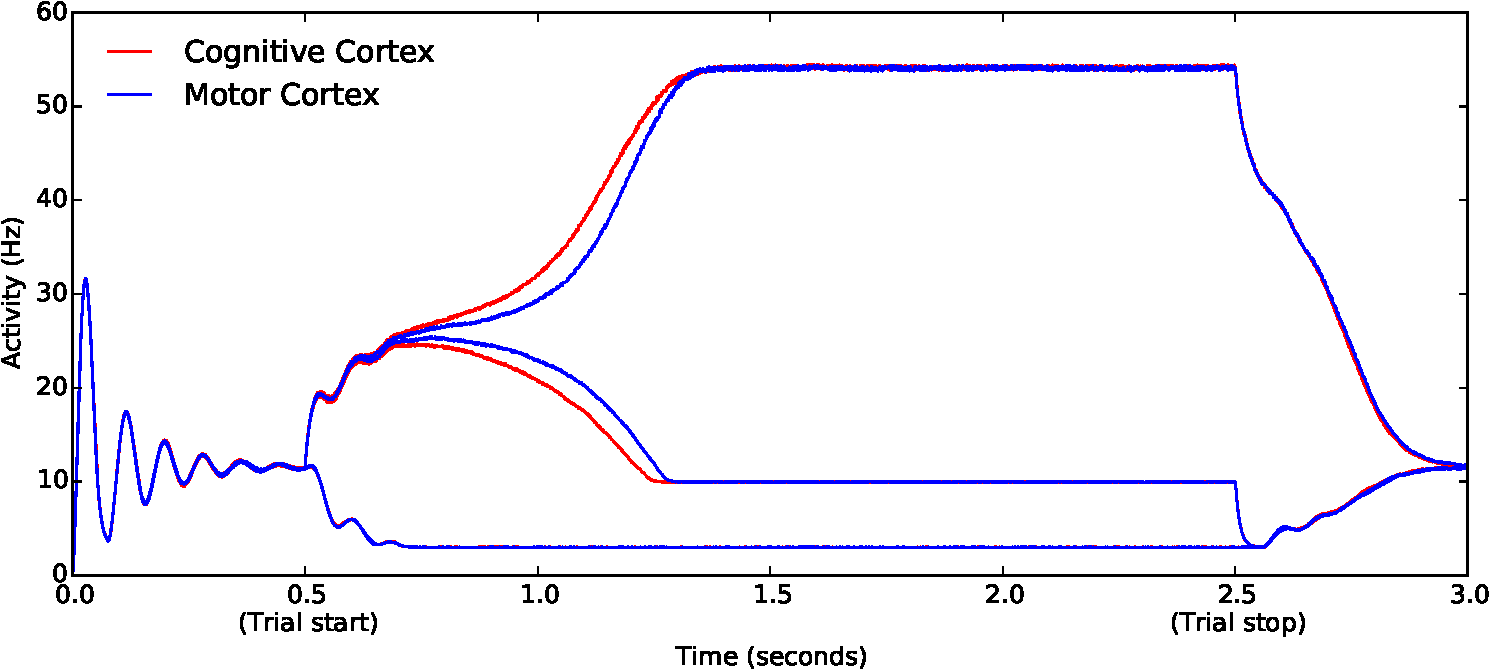
\includegraphics[width=\textwidth]{./figure-1.pdf}
  \caption{\textbf{Activity in the cortical population during a single
      trial of action selection.} This is the reproduction of figure 4 of the
    original article.}
  \label{fig:1}
\end{figure}
%
We also test learning capacity of the model by reproducing the same
procedure as in the original article (250 experiments, 120 trials) but
we used a modified and simpler learning rule (see Plasiticity table)
since the original learning rule used a sigmodial transfer function but
no actual details were given on how to enforce it.
%
\begin{figure}[htbp]
  \centering
  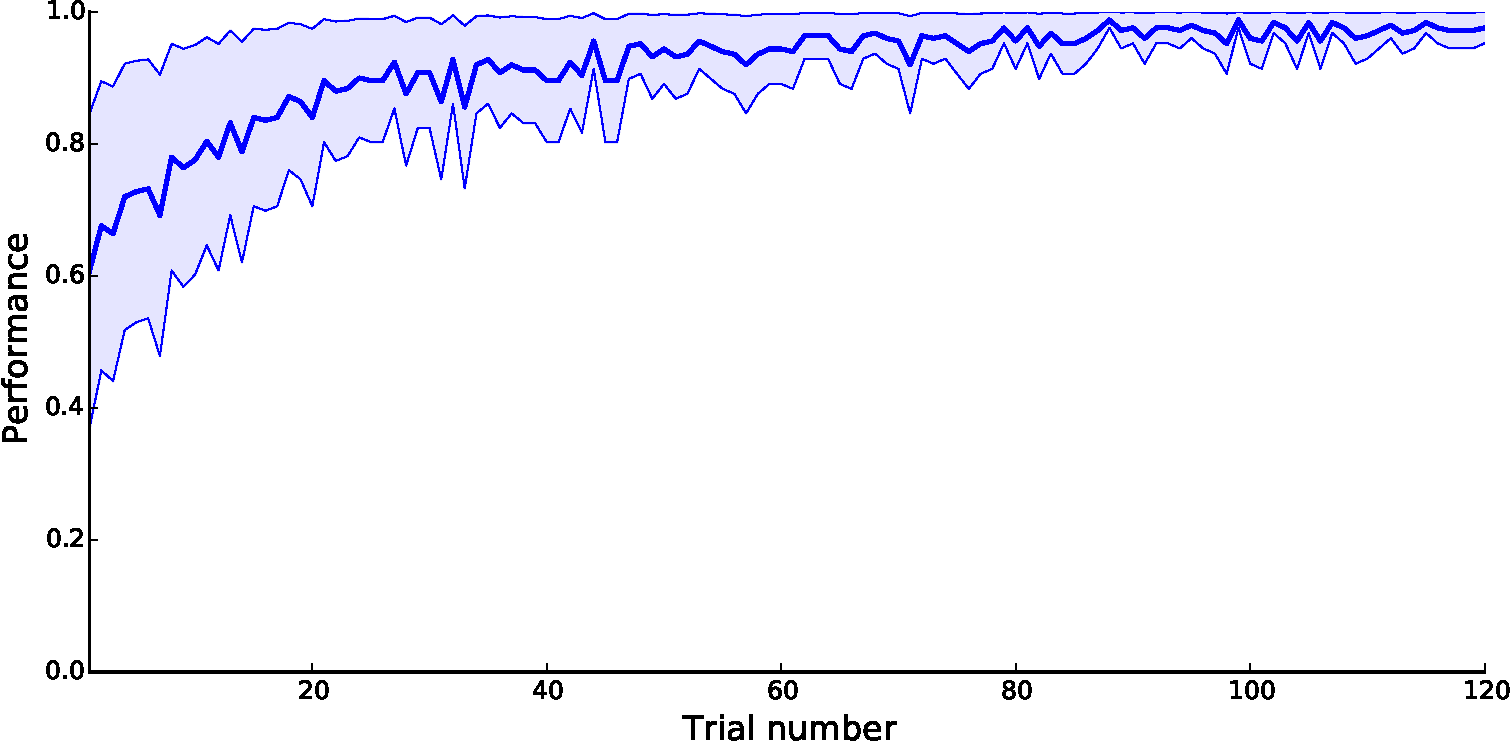
\includegraphics[width=\textwidth]{./figure-2.pdf}
  \caption{\textbf{Learning time course over 120 trials, averaged over 250
      simulations.} The blue filled area indicates the variance of the mean
    performance.}
\end{figure}

\section* {Conclusion}

We were able to reproduce original results, confirming the correctness of the
original implementation of the model.
